\section{Recursió vs Iteració}

Per entendre tòpics que veurem més endavant com la programació dinàmica entre altres, primer hem d'entendre la recursió i la iteració (és totalment normal que costi d'entendre i que necessitis llegir-ho vàries vegades per entendre el funcionament d'aquesta). \newline

La recursió és un algoritme el qual conté una funció que és crida a ella mateixa (funció recursiva), és utilitzada per resoldre petits subproblemes del problema original i generalment la funció consta de dos casos. \newline

Cas base -> finalitza la recursió.
Cas recursiu -> continua la recursió. \newline

La iteració és un recurs que s'empra en quasi tots els problemes de programació i es basa en una seqüència d'instruccions o codi que es repeteixen fins que s'arriba a un resultat final específic.
Per iterar en la majoria de llenguatges de programació s'usen bucles "for". \newline

Sovint els problemes es poden resoldre amb les dues tècniques (recursió i iteració) però depenent de la situació preferirem fer servir una o l'altra. \newline

Un exemple molt típic de l'ús de la recursió i iteració és quan volem trobar el valor de la posició n de la seqüència de Fibonacci. \newline

La seqüència de Fibonacci és una seqüència infinita de nombres naturals; a partir del 0 i l'1, es van sumant per parelles, de tal manera que cada nombre menys els primers dos de la seqüència (0,1) és igual a la suma dels dos anteriors nombres. \newline

EX: 0, 1, 1, 2, 3, 5, 8, 13, 21, 34, 55... \newline

\begin{center}
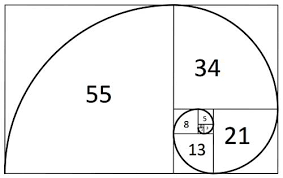
\includegraphics[width= .6 \textwidth]{fib.png}
\end{center}

\newpage

Donada qualsevol $n$ tal que $n$ és la posició del nombre en la seqüència, amb l'ús de la recursió podem trobar el nombre el qual la seva posició en la seqüència és $n$.

Per tant, el que farem és recursivament, cridar la funció $fib$ i retornar la suma de $fib(n - 1)$ + $fib(n - 2)$, ja que $n$ és igual a la suma dels dos anteriors, el nostre cas base serà quan $n$ sigui igual a 1 o 0 i llavors haurem de retornar 1 o 0 respectivament, puix que voldrà dir que hem arribat al final de la seqüència. \newline

Així i tot, això també ho podem fer amb l'ús de la iteració, simplement emmagatzemem els valors de la seqüència en un vector i a cada pas, $f[j] = f[j-1] + f[j-2]$, on f representa el vector on guardem els valors i $j$ té un valor d'entre $2 <= j < \infty$, ja que $f[0] = 0$ i $f[1] = 1$. \newline

A continuació podem observar el càlcul del valor de la seqüència de Fibonacci en la posició $n$, en el primer codi fem servir la recursió i en el segon utilitzem la iteració. \newline

\begin{lstlisting}
int fib(int n){
    if (n <= 1) // cas base
        return n;
    return fib(n - 1) + fib(n - 2); // cas recursiu
}

int main(){
    cout << "Introdueix n: " << endl;
    int n; // Input -> 9
    cin >> n;
    cout << fib(n); // Output -> 34
}
\end{lstlisting}

\begin{lstlisting}
int fib(int n){
    vector f(n+2); // llista on guardem els valors
    f[0] = 0;
    f[1] = 1;
    
    for (int i = 2; i <= n; i++){ // iteració
        f[i] = f[i-1] + f[i-2];
    }
    return f[n];
}

int main(){
    int n; // Input -> 9
    cin >> n;
    cout << fib(n); // Output -> 34
}
\end{lstlisting}

Cal recalcar que el codi que usa recursió té una complexitat temporal de $O(2^n)$, en canvi, el codi que utilitza iteració té una complexitat temporal de $O(n)$.

Si $n = 50$, aquest el nombre d'operacions que faria l'ordinador amb les diferents tècniques: \newline

\underline{Operacions recursió} -> $2^{50}$ = $1,256*10^{15}$ operacions. \newline

\underline{Operacions iteració} -> $50 = 50$ operacions. \newline

Com podem veure, la iteració en general té una complexitat més baixa que la recursió i, per tant, un més bon rendiment. \newline

En la següent imatge podem veure totes les crides recursives que realitza el codi que empra la recursió, podem observar que hi ha crides repetides i que es poden optimitzar, aquesta optimització es pot realitzar fàcilment amb la programació dinàmica. \newline

\begin{center}
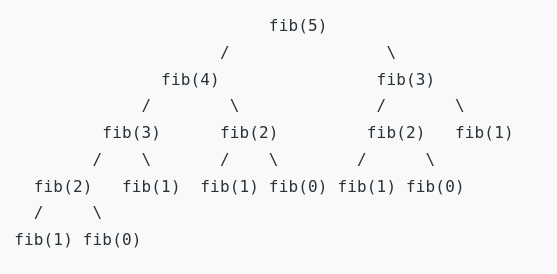
\includegraphics[width=.9 \textwidth]{crides.png}
\end{center}

(La branca de fib(3) i fib(2) està repetida)

